%! Author = tstreule

\section{Molecular Adsorption and Electron Transfer}
%%%%%%%%%%%%%%%%%%%%%%%%%%%%%%%%%%%%%%%%%%%%%%%%%%%%%%
%%%%%%%%%%%%%%%%%%%%%%%%%%%%%%%%%%%%%%%%%%%%%%%%%%%%%%
\subsection{Quantum Mechanics}
%
\formula{Schrödinger eq.}{\hat{H}\psi(\vec{r}) = E\psi(\vec{r})}
\quad where $\hat{H} = -\frac{\hbar}{2m}\pderiv[2]{~}{x} + V$

\formula{\textbf{1D potential well}}{\psi(x) = \sqrt{\frac{2}{L}} \sin(k_nx)}
\quad for $0\leq x\leq L$
\formtex{~}{where $k_n = \frac{n\pi}{L}$, $n\in\mathbb{N}$ and $E_n = \frac{\hbar^2k_n^2}{2m}$}

\formula{\textbf{1D potential barrier} (tunneling)}{
    \psi(x) =
    \begin{cases}
        A\eu^{\iu k'x} + B\eu^{-\iu k'x}	& \phantom{for } x\leq0\\
        C\eu^{\iu k''x} + D\eu^{-\iu k''x}	& \text{for }    0\leq x\leq d\\
        F\eu^{\iu k'x}						& \phantom{for } \text{otw.}
    \end{cases}
}
\formtex{~}{where $k' =\sqrt{2mE}/\hbar$ and $k''\!\!=\sqrt{2m(V_0\!-\!E)}/\hbar$}

\formbox{transm./tunneling probability}{T = \frac{F^*\!F}{A^*\!A} = B\eu^{-\beta d}}
, $\beta {=} {-}2\sqrt{2m(V_0{-}E)}/\hbar$
%%%%%%%%%%%%%%%%%%%%%%%%%%%%%%%%%%%%%%%%%%%%%%%%%%%%%%
\subsection{Electronic Transport through Molecules}
%
\formbox{Quantum conductance (1D)}{G = G_0\cdot T}
\enskip $G_0 = \frac{2e^2}{h}$,
\enskip in parallel: $G = N\cdot G_0$
\formbox{Tunneling probability}{T = B\eu^{-\beta d}}
$\propto\;\;\; \eu^{-\beta d} = \left(\eu^{-\beta_{N\!P}d}\right)^N$
\formbox{1D channel current}{j = {-}(\mu_1{-}\mu_2)e\;v\;\rho_E}
\enskip $\rho_E {=} DOS {=} \frac{1}{\hbar\pi}\sqrt{2m/E}$
%%%%%%%%%%%%%%%%%%%%%%%%%%%%%%%%%%%%%%%%%%%%%%%%%%%%%%
\subsection{Atomic and Molecular Orbitals}
%
%	The linear combination of atomic orbitals (\textbf{LCAO}) approximation supposes that molecular orbitals can be constructed from linear superpositions of atomic orbitals centred on individual atoms.\\
%	IMPORTANT: linear combinations of n atomic orbitals each with its own energy level (even if of the same E value!!!) give rise to n energy levels.
%
\textbf{Bond order}: defined by difference (\#electrons) divided by two\\
$\to$ If the bond order is different from zero, then the bond is \textit{stable}
%
%	\textbf{HOMO - LUMO} (highest occupied vs lowest unoccupied MO):\\
%	If we add thermal energy, the electrons will begin to jump. Since all lower states are filled, the first electron will jump from HOMO to LUMO.
%%%%%%%%%%%%%%%%%%%%%%%%%%%%%%%%%%%%%%%%%%%%%%%%%%%%%%
%	\subsection{Electrical Biosensor}
%	%
%	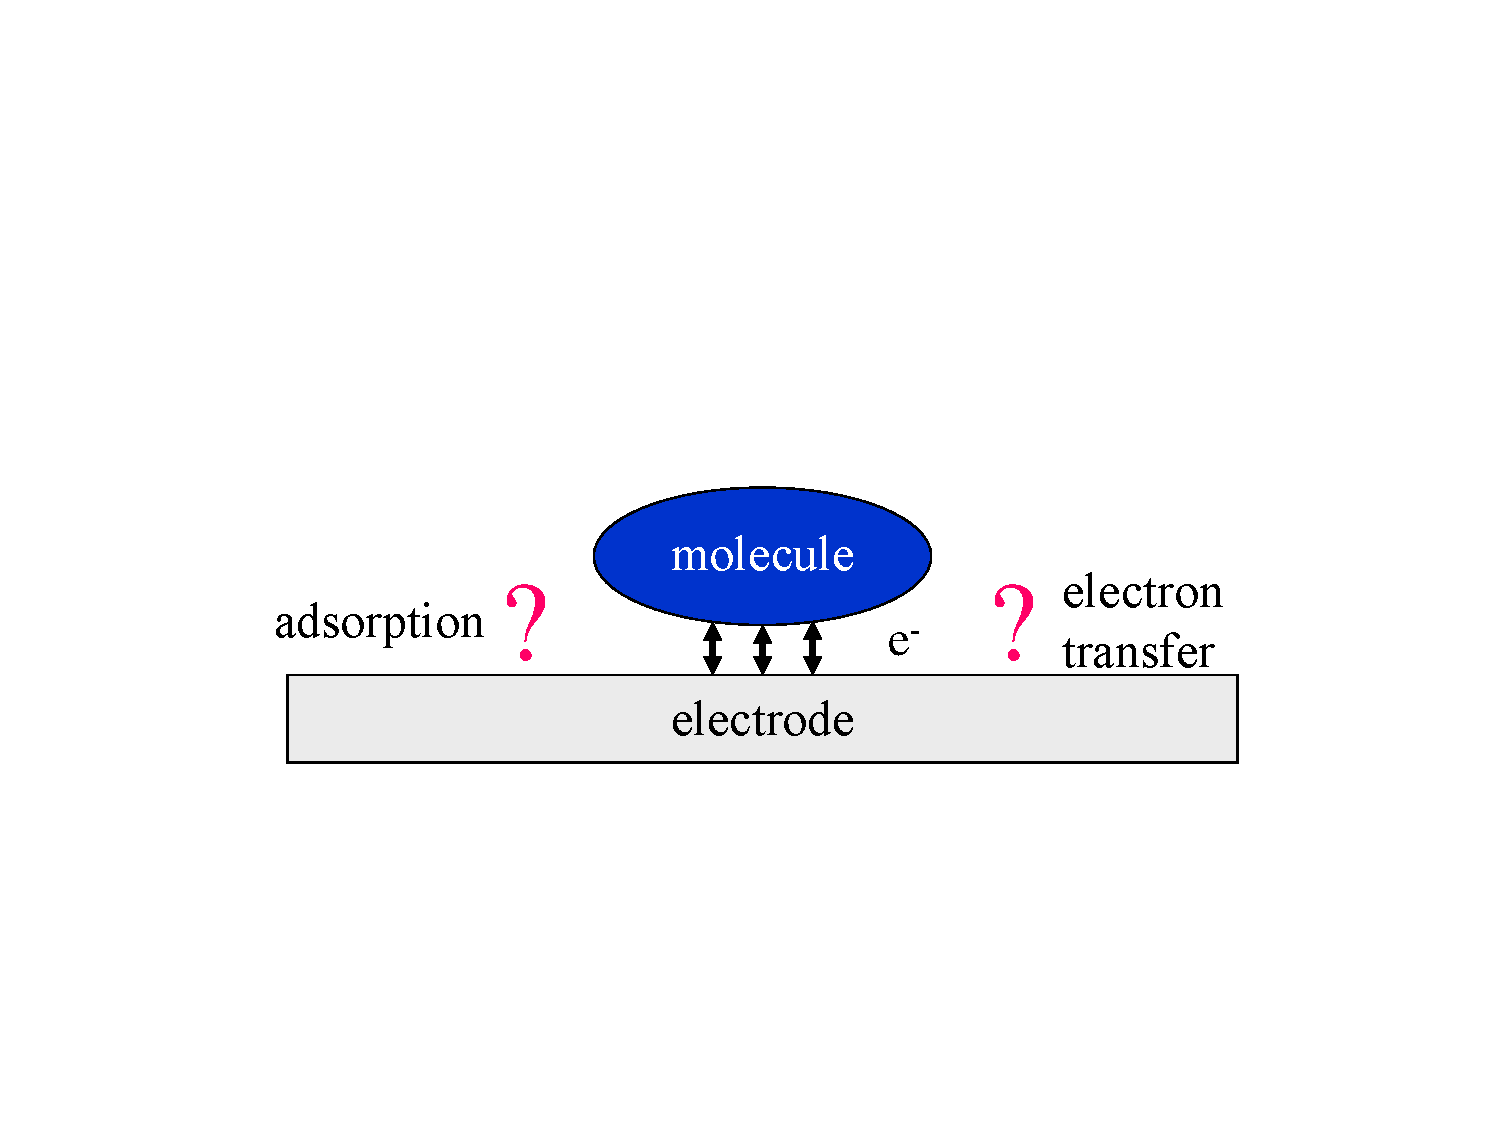
\includegraphics[width=.5\columnwidth]{Electrical_Biosensor}
%%%%%%%%%%%%%%%%%%%%%%%%%%%%%%%%%%%%%%%%%%%%%%%%%%%%%%
\subsection{Transition State Theory \textnormal{$A+B \to [AB] \to C+D$}}
%
%	Criterion is that colliding molecules must have sufficient energy to overcome a potential energy barrier (the activation energy) to react.
%
\formula{Gibbs free energy}{G = H - TS = U + pV - TS}
\formbox{\textbf{Ideal gas law}}{pV = n\ped{total}RT}
\vspace{-1mm}
%%%%%%%%%%%%%%%%%%%%%%%%%%%%%%%%%%%%%%%%%%%%%%%%%%%%%%
\subsubsection{Marcus Theory}
%
\begin{minipage}{.5\columnwidth}
    \includegraphics[width=.8\columnwidth]{Electrochemistry_Marcus_Theory}
\end{minipage}%
\begin{minipage}{.5\columnwidth}
    See \textbf{section \ref{sec:butler-volmer}} (Butler-Volmer)\par
    \begin{tabular}{r@{$\;=\;$}l}
        $k\ped{red}$	& $v\ped{red} \; \eu^{-\frac{\Delta^\ddagger G\ped{red}}{RT}}$\\
        $k\ped{ox}$		& $v\ped{ox}  \; \eu^{-\frac{\Delta^\ddagger G\ped{ox}}{RT}}$\\
        \addlinespace
        $\Delta^\ddagger G\ped{red}$	& $\!\!~^\ddagger G-G\ped{ox,min}$\\
        $\Delta^\ddagger G\ped{ox}$	& $\!\!~^\ddagger G-G\ped{red,min}$
    \end{tabular}
\end{minipage}
%
%	\formula{rate constant}{k_{et} \propto \eu^{-\frac{\Delta^\ddagger G}{RT}}}
%		\quad with \quad $R = k_B N_A = \unit[8.3]{J\;K^{-1}mol^{-1}}$
%%%%%%%%%%%%%%%%%%%%%%%%%%%%%%%%%%%%%%%%%%%%%%%%%%%%%%
\subsubsection{Gerischer's view}
%
\begin{minipage}{.4\columnwidth}
    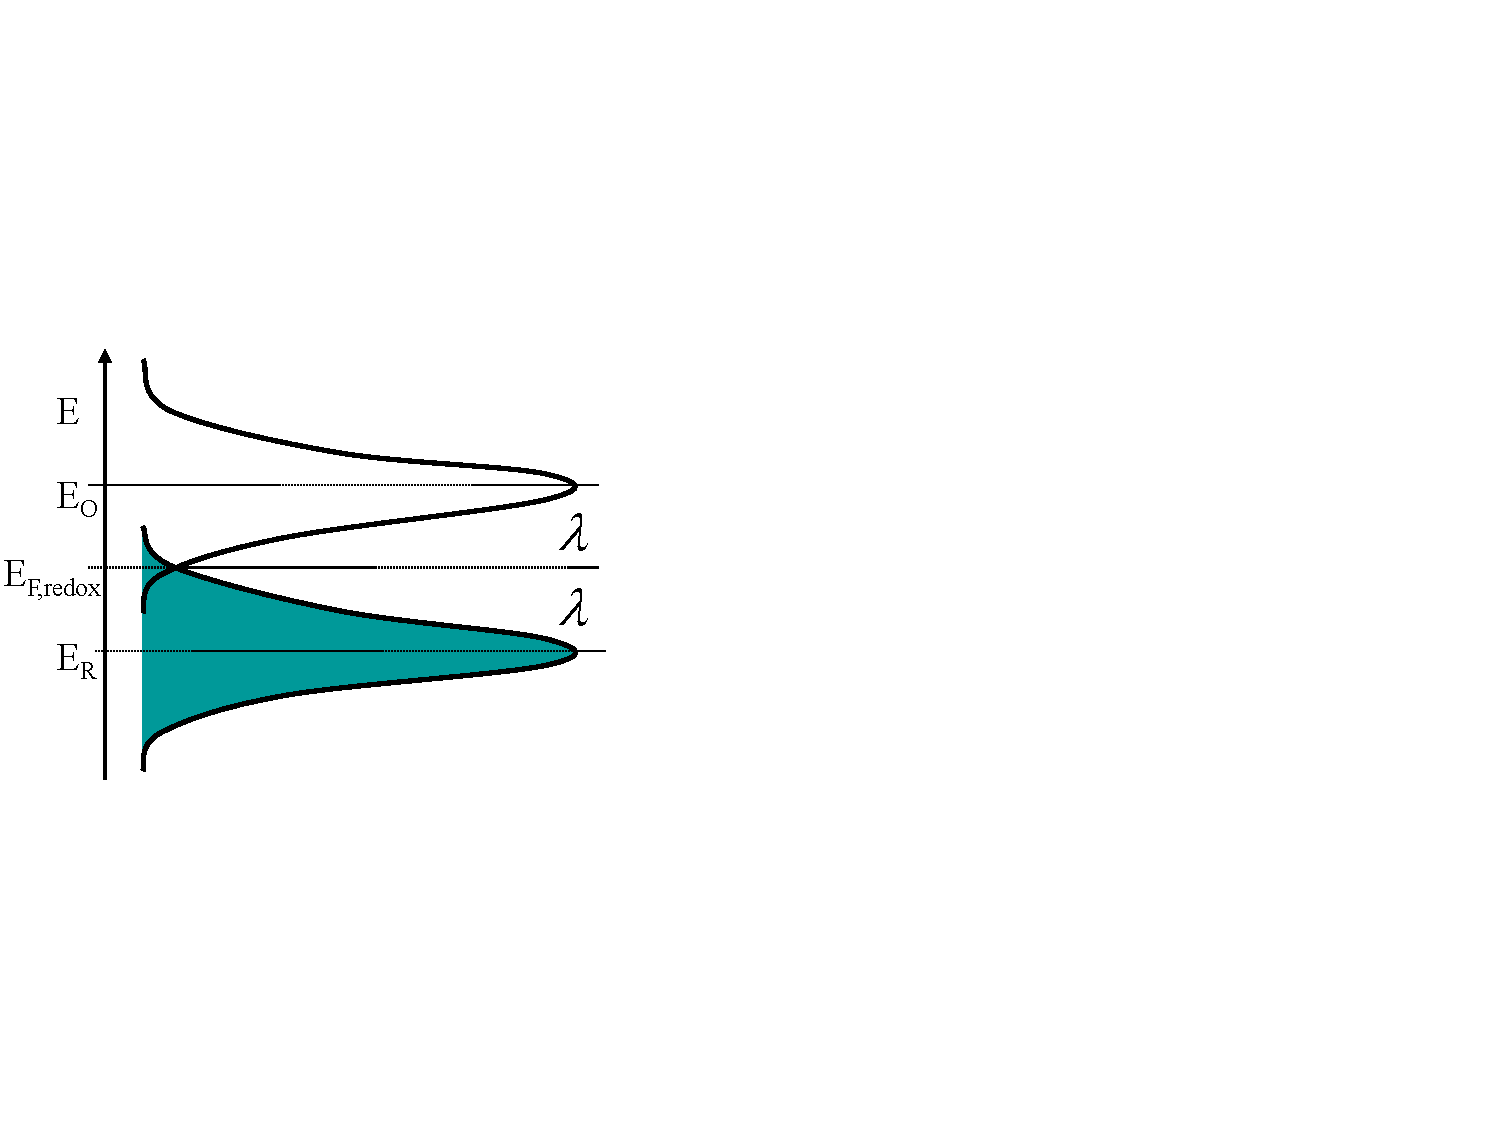
\includegraphics[width=\columnwidth]{Redox_Energy_Levels_1}%
    \hspace{-.6\columnwidth}
    \parbox[b]{.4\columnwidth}{
        $D\ped{ox}(\lambda,E)$ \vspace{20mm}\\\vspace{2mm}
        $D\ped{red}(\lambda,E)$
    }
\end{minipage}%
\begin{minipage}{.15\columnwidth}
    \centering
    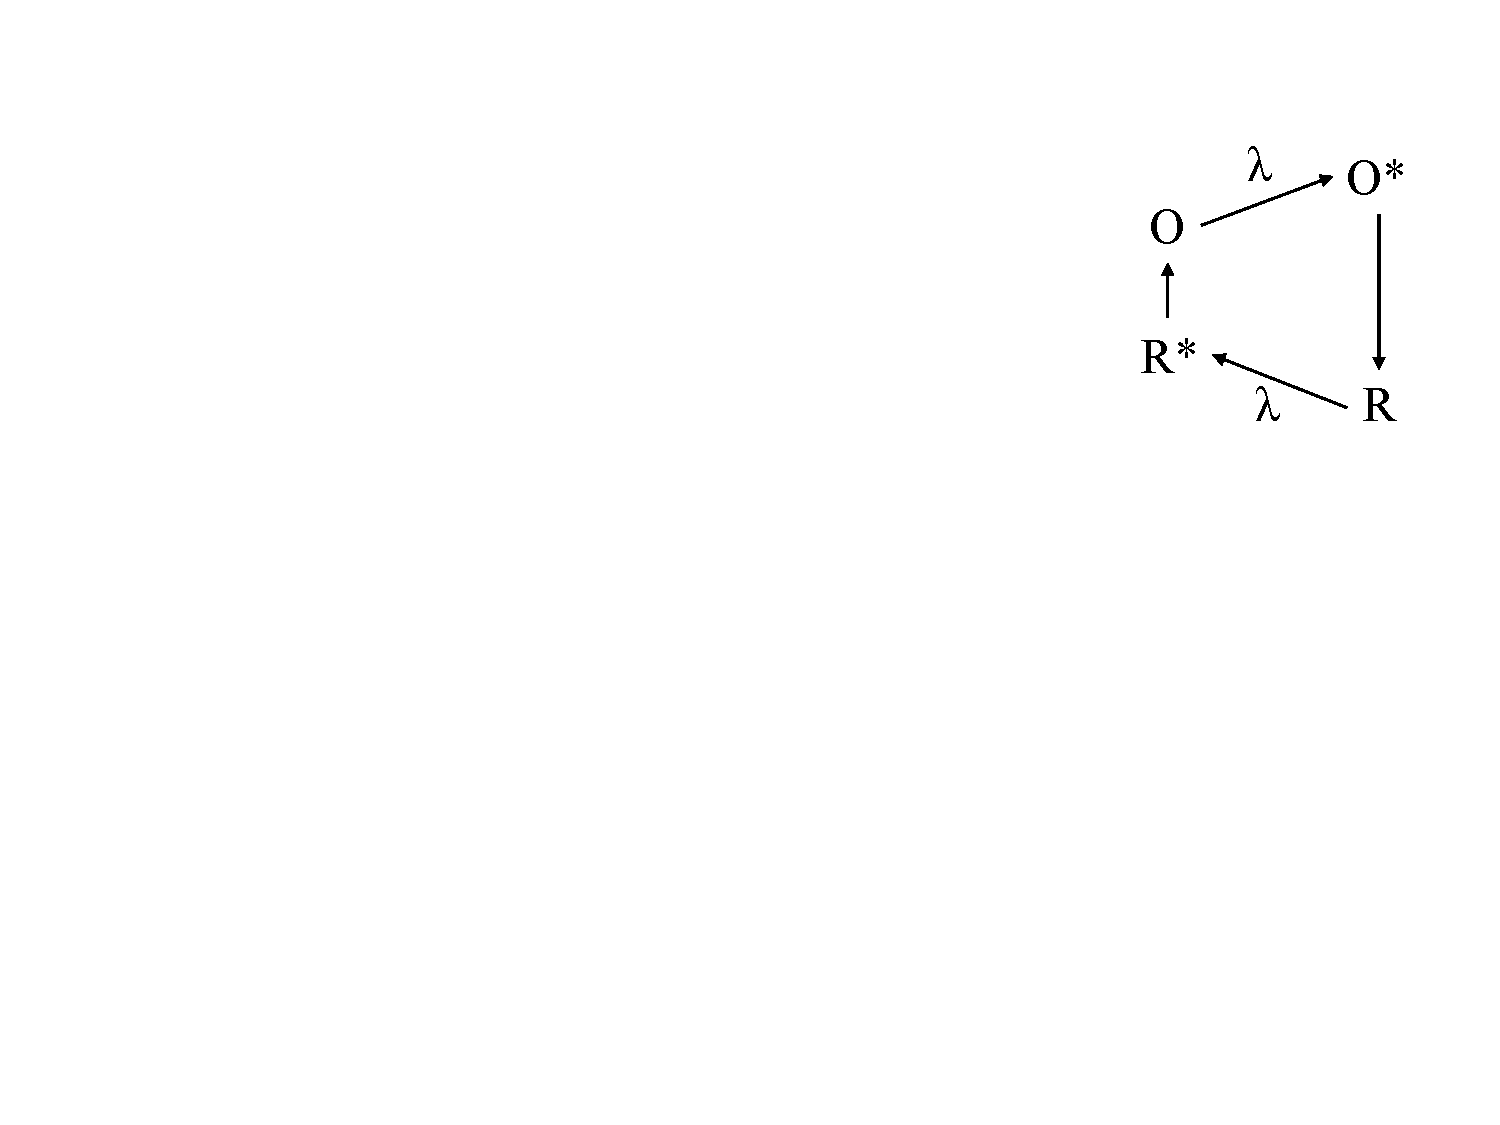
\includegraphics[width=.9\columnwidth]{Redox_Energy_Levels_2}
\end{minipage}%
\begin{minipage}{.45\columnwidth}
    \quad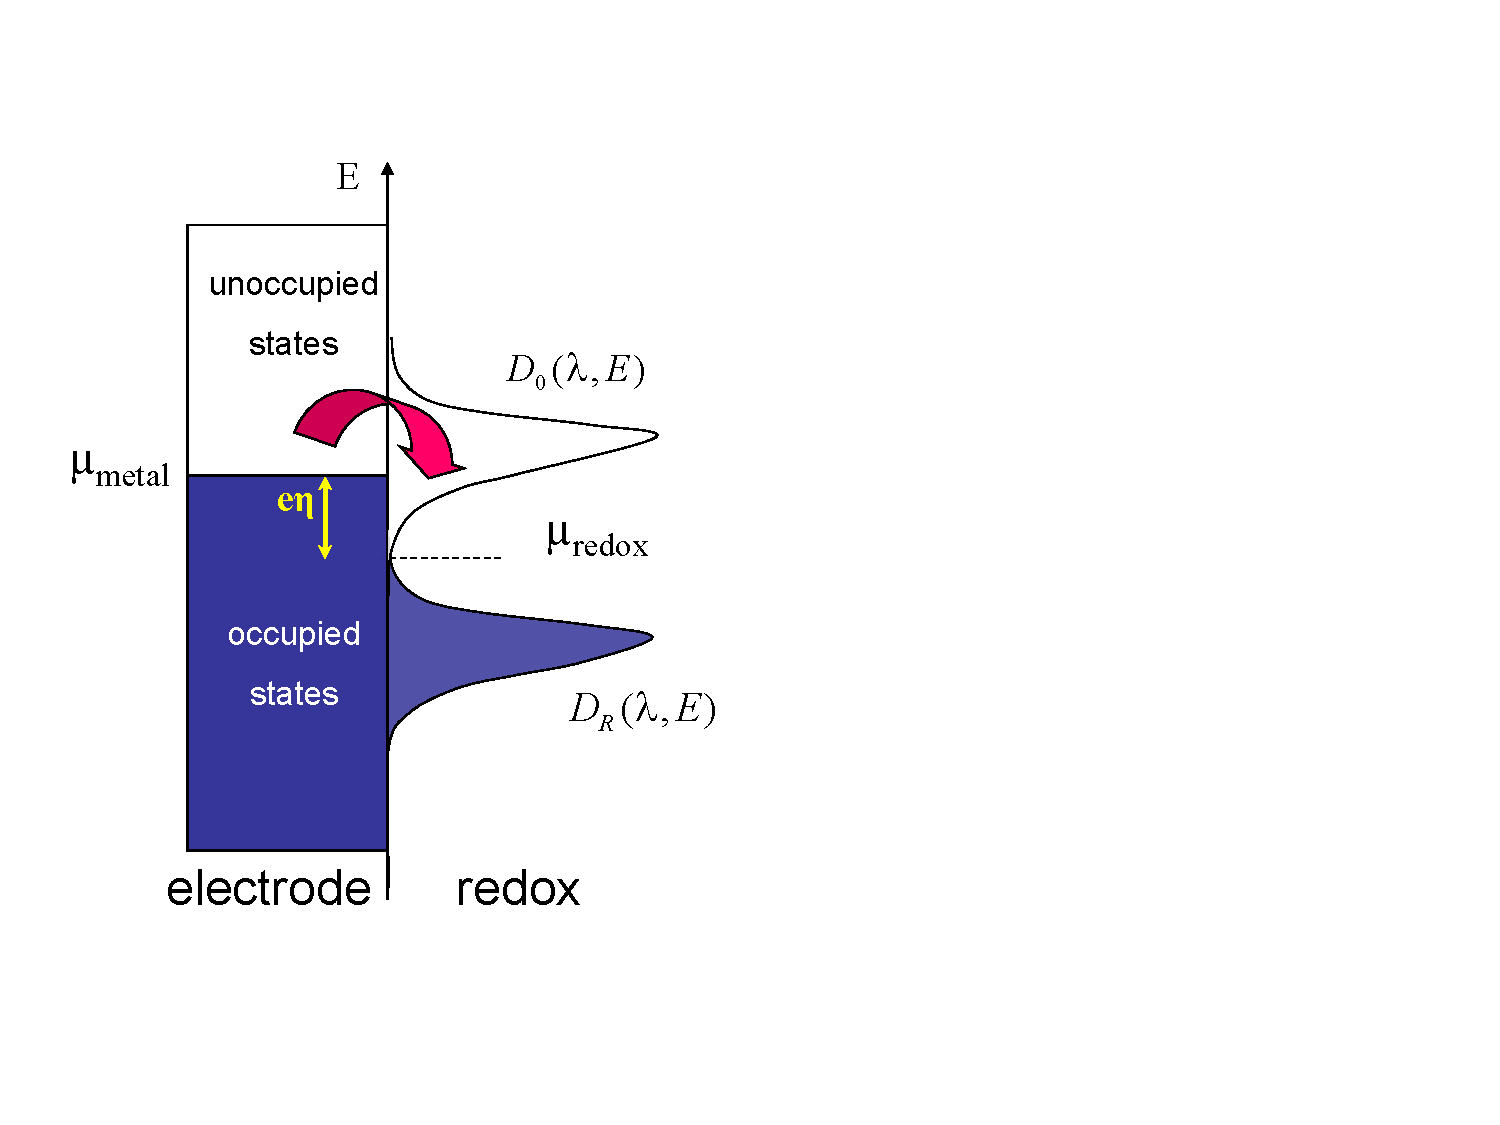
\includegraphics[width=.55\columnwidth]{Electrochemistry_Gerischers_View_Cathodic}%
    \hfill\hspace{-\columnwidth}
    \parbox[b]{\columnwidth}{
        \hfill \textbf{cathodic} polariz. \par
        \hfill $i^+ \gg i^-$\vspace{22mm}\\
    }
%		Gaussian curve: ($+$: red, $-$: ox)\\
%		$W\ped{red/ox} = \frac{1}{\sqrt{4\pi\lambda k\ped{B}T}} \eu^{-\frac{(E-E_F\pm\lambda)^2}{4\lambda k\ped{B}T}}$
\end{minipage}
